% $Revision$
% $Id$

\chapter{Lexical Structure} \label{lexical structure}

\section{Notational Conventions}

In this and the subsequent chapters, subsets of the \frege{} grammar are given in running text. The complete grammar is the set of rules that is the union of all those subsets.

\par A
grammar rule defines a nonterminal symbol as a sequence composed of terminal symbols, nonterminal symbols or subrules indicating that the enclosed sequence \opt{is optional} or may occur \some{zero or more} times.
Nonterminal symbols and variable terminal symbols are written in \nont{italics}, constant terminals in bold \term{typewriter} font.
The definition of a nonterminal starts in the left margin and may
consist of alternative rules. Alternatives are separated by a
line break, some indent and a vertical bar.

\par In this section particularly, the lexical syntax of terminal symbols of the grammar will be defined by regular expression.
\index{expression!regular}
We use regular expressions as defined in the documentation of class
\texttt{java.util.regex.Pattern} in \cite{apidoc}. Regular expression
will appear in coloured typewriter font like this
\regex{$\backslash{}$s?}.

In order to make things more readable, sometimes the name of a terminal symbol is used in a regular expression. The meaning is here to replace the terminal symbol with the regular expression defining it. For example:

\begin{flushleft}
\rul{digits}  \regex{$\backslash{}$d+}\\
\rul{float}   \term{digits}\regex{($\backslash{}$.}\term{digits}\regex{)?}\\
This is the same as:\\
\rul{float} \regex{$\backslash{}$d+($\backslash{}$.$\backslash{}$d+)?}
\end{flushleft}

Likewise, instead of \regex{foo|bar} we sometimes write \regex{foo}\oder{}\regex{bar}.

All regular expressions are to be understood to be anchored at the start of the yet unprocessed portion of the program text.

\par Some symbols like parentheses, separators and so on stand for themselves and are specified verbatim each time they occur in the grammar. To distinguish verbatim symbols like \sym{<- , ; ::} etc. from meta-syntactical symbols such as {\Large $|$} and \opt{..} and from regular expressions, we write them in a different colour.

\begin{figure}[bth]
\epsfxsize\hsize \epsfbox{utfcode.eps}
%\centering
%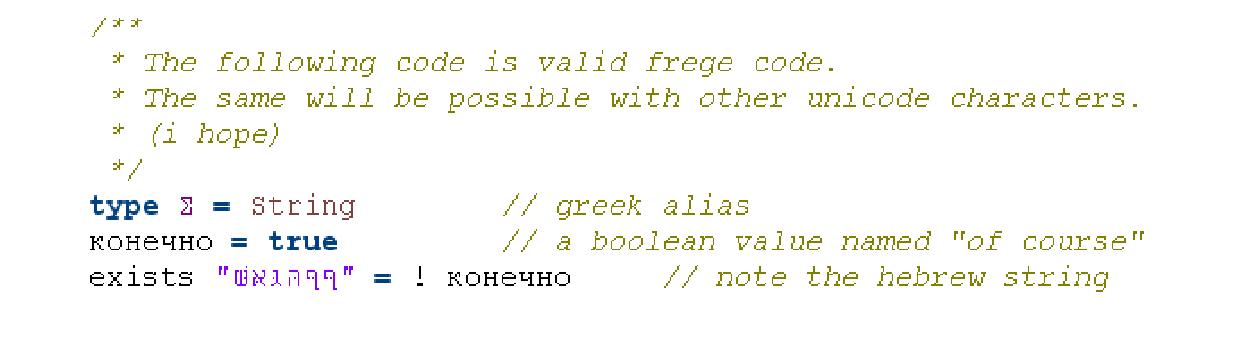
\includegraphics{utfcode}
\caption{\frege{} code with greek, cyrillic and hebrew letters}
\label{utf8}
\end{figure}

\par \frege{} uses the Unicode character set, see \autoref{utf8} for an
example. 
%However, the syntactically relvant characters are drawn from
%the ASCII character set only. The same holds for most names and operators defined in
%the standard libraries. \index{character set!Unicode}

Compilers will support program text stored in files with encodings
that are supported by the \java{} platform. The standard encoding is UTF8.
For detailed information consult the \java{}
API documentation \cite{apidoc}. \index{character!encoding}

While it is possible to compose names and operator symbols from
valid unicode symbols, one should keep in mind that extensive use of
this feature will make the program text
difficult, if not impossible, to understand for members of different
cultural background.

\section{Lexical program structure}

\begin{flushleft}
\rul{program} \some{\nont{line}}\\
\rul{line} \some{\nont{whitespace} \nont{token}} \nont{whitespace}\\
\rul{whitespace} \regex{$\backslash{}$s*}\\
\rul{token} \nont{varid} \oder \nont{conid} \oder \nont{keyword} \oder \nont{qualifier} \oder \nont{parentheses} \oder \nont{specialsym}
\\\hspace{0.5in} \oder \nont{lexop} \oder \nont{literal}
\end{flushleft}

A program is made up of lines.
Source code is broken into lines before tokenization by appropriate
input reading functions that will recognize and strip line separator
characters typical for the underlying operating system. 

With the exception of \hyperref[doccomment]{documentation text} there is no token that would
extend over more than one line.

Each line contains zero or more tokens separated by whitespace. Still
more whitespace can occur before the first token or after the last
token.

Note that the definition of \nont{whitespace} allows for the empty
string of whitespace characters. Consequently, tokens may appear not to
be separated at all.

The possibility of zero length whitespace does not mean that whitespace
may be dismissed altogether. On the contrary, whenever two tokens appear
in sequence where a non empty prefix of the second token might also be a
valid suffix of the first one, nonempty whitespace is required to allow
for unambiguous tokenization. In other words, the tokenization algorithm
will recognize the longest prefix of the remaining characters on the
current line that form a valid token.

Consider the following example:
\example{\par
  a+2\\
  a2\\
  a 2\\
  a\\
 2
}
There are 3 tokens in the first line and one token in the second line.
Since a digit is a valid suffix of an identifier, a space must occur
between a and 2 to obtain two tokens, as shown on the third line.
Another possibility to separate the tokens would be to write them on
different lines, as shown in the last two lines.

\section{Comments} \index{comment}

Comments can appear everywhere whitespace can.

\begin{flushleft}
\rul{comment} \nont{linecomment} \oder{} \nont{blockcomment}\\
\rul{linecomment} \regex{---?.*} \gcom{line comment extends to end of line}\\
\rul{blockcomment} \regex{(?s)$\backslash$\{--?.*-$\backslash$\}}\\
\end{flushleft}

Note that the character sequence making up a block comment may extend over multiple lines
\footnote{This is the only exception to the rule that no token crosses line
boundaries.}.

If some code is commented out using a block comment, then any occurrence of  \regex{-\}} within 
a string or within a line comment in that code will terminate the comment.  

\hasdiff{\\
Block comments do not nest. A user defined operator (see \autoref{operator}) must not start with the characters \texttt{\{-} or \texttt{--}.
}

\subsection{Documentation Text} \label{doccomment} \index{comment!documentation}

Block comments starting with \regex{\{--} and line comments starting with  \regex{---} are treated as \textit{documentation text}.
Unlike an ordinary comment, a documentation text is a token and hence is not only lexically but also syntactically relevant.

There are only certain places where documentation text may appear, as will be detailed in this section. 
In order not to complicate matters, subsequent sections will not mention documentation text anymore.

A documentation text may appear:
\begin{enumerate}
\item before the \term{package} keyword that starts a package. This will be the documentation for the package.
\item in place of a \hyperref[declarations]{top level declaration} or a declaration in the \term{where} clause of a data, class or instance declaration. It can also appear immediately before such a declaration.
This will be the documentation for the subsequent declared item. 
\item immediately either before or after a \nont{constructor} in a \hyperref[algdcl]{data declaration}. This will be the documentation for that constructor.
\item immediately before or after a constructor field. In the latter case, no comma must be written before the next constructor field. 
\end{enumerate}

For convenience, in cases 1 and 2 a sequence of documentation comments optionally separated by semicolon can be written.
The text of the documentation comments will be concatenated with an interleaving paragraph break.

\example{
\begin{flushleft}
--- this package is documented\\
\{-- second paragraph of package doc -\}\\
\{-- third paragraph of package doc-\}\\
package D where\\
\\
--- this is the list of Fibonacci numbers\\
fib = 1:1:zipWith (+) fib (tail fib)\\
--- document type D\\
data D = \\
\hspace{1cm}--- document constructor C\\
\hspace{1cm} C \{ name :: String --- document name, no comma here\\
\hspace{2cm}\{-- document age -\}\\
\hspace{2cm}age :: Int \}\\
\hspace{1cm}$|$ N\hspace{1cm}--- document costructor N\\
\end{flushleft}
}

Documentation text will be copied verbatim and it will be available in the binary results of compilation (e.g. \java{} class files), so that documentation processing tools can access it to generate documentation in various formats.


\section{Identifiers and Keywords} \index{identifier} \label {qualified names}

\begin{flushleft}

\rul{qualifier}
\regex{($\backslash$p\{Lu\}($\backslash$d$|$\_$|\backslash$p\{L\})*$\backslash$.)\{1,2\}
}\\

\rul{varid} \regex{$\backslash$p\{Ll\}($\backslash$d$|$\_$|\backslash$p\{L\})*'*}\\

\rul{conid} \regex{$\backslash$p\{Lu\}($\backslash$d$|$\_$|\backslash$p\{L\})*}\\

\rul{qvarid} \nont{qualifier} \nont{varid} \oder{} \nont{varid}\\
\rul{qconid} \nont{qualifier} \nont{conid} \oder{} \nont{conid}\\
\end{flushleft}

These rather complicated regular expressions deserve some further
explanation.

We distinguish lexically between two classes of identifiers.
Names for functions, values and local variables are \nont{varid}s
and start with a lowercase letter.
Names that start with an uppercase letter (\nont{conid})
stand for value constructors,
type constructors, type classes, type alises or name spaces.

Sometimes it is necessary to name an item that is defined in another
package or in the scope of a type or type class. Thus we need qualified
names, defined here as \nont{qvarid} and \nont{qconid}. They are formed
by writing a \nont{qualifier} before a \nont{varid} or \nont{conid}.

A \nont{qualifier} consists of one or two identifiers starting
with an uppercase letter, where each identifier is immediately
followed by a dot. The identifiers denote name spaces, types or type
classes. A \nont{qualifier} like \texttt{Foo.Bar.} is a single
token and thus may not contain spaces.

The syntax ensures that qualifiers will
only be used to form qualified names and will
thus always be followed by either a
\nont{varid} or a \nont{conid}. Hence, we have lexically and syntactically
enforced, that a reference to an item will be one of
the following:

\ex{
$N$.$T$.$v$ \hspace{0.3cm} $N$.$T$.$C$ \\
$T$.$v$  \hspace{0.3cm} $T$.$C$ \hspace{0.3cm}
$N$.$v$  \hspace{0.3cm} $N$.$C$ \hspace{0.3cm} $N$.$T$ \\
$v$ \hspace{0.3cm} $C$ \hspace{0.3cm} $T$
}

where $N$ would be a name space, $T$ a type or class name, $C$ a
data constructor name and $v$ the name of a function or pattern binding.

There are rare cases where it is possible to confuse the dots in the qualifiers with
the special operator \texttt{.} explained later, an example can be found  \hyperref[confusedots]{here}. 
Fortunately, such constructs can be disambiguated with spaces or parentheses.

\note{Unlike in other languages, a \frege{} identifier cannot start with
an underscore.}

\subsubsection{Name Resolution and Scope}

Names appearing in expressions and types are resolved by the following rules, where $N$, $T$ and $C$ stand for \nont{conid}s and $v$ for \nont{varid}s:

\begin{description}
\item [Names of the form $v$] every enclosing lexical scope provided by a \term{let}, lambda expression or case alternative is searched in turn for the name.  If it is found, then it refers to an item defined in a \term{let} expression or a (part of a) pattern in a lambda expression or case alternative. Otherwise, it must be a globally visible item. If $v$ appears in the scope of a data definition, class definition or instance definition and there is a variable or function binding with the name $v$ then it is resolved to mean this binding. Otherwise, it must be a global function or variable binding or a class member.
\item [Names of the form $T$ or $C$] $T$ may appear in type signatures, where it denotes type constructors, type names or class names, either imported ones or ones that are declared in the current package. In expressions and patterns, $C$ denotes a value constructor.
\item[Names of the form $N$.$T$ or $N$.$C$] $N$ must be a name space denoting an imported package, a data type or a class. $T$ must be a class name, type name or $C$ must be a data constructor from this name space. While it is possible, that a type and a data constructor have the same name this does not introduce ambiguities because syntactically either a type name $T$ or a data constructor $C$ can be meant, but not both.

It is also possible that a type name and a name space of an imported package have the same name. In this case, only the name space of the imported package is searched. If one needs to access $C$ in the name space of the type $N.N$ one needs to write a qualified name of the form ($N$.$N$.$C$).
\item[Names of the form $N$.$v$]
$N$ must be name space denoting an imported package, a data type or a class.
$v$ is the name of a function or pattern binding in $N$. Again, if there is a namespace $N$ and a type $T$ and $N = T$, then only $N$ is searched.
\item[Names of the form $N$.$T$.$C$ or $N$.$T$.$v$] denote a function or pattern binding or a data constructor belonging to type or class $T$ from name space $N$.
\end{description}

\subsubsection{Keywords}

Some character sequences that would otherwise be matched by rule \nont{varid} are keywords and will be recognized by the scanner as distinct terminal symbols.

\begin{flushleft}
\label{keyword} \index{keyword}
\term{abstract}: \regex{abstract} \\
%\term{break}: \regex{break} \\
\term{case}: \regex{case} \\
\term{class}: \regex{class|interface}\\
%\term{continue}: \regex{continue} \\
\term{data}: \regex{data} \\
\term{derive}: \regex{derive} \\
\term{do}: \regex{do} \\
\term{else}: \regex{else} \\
%\term{extends}: \regex{extends} \\
\term{false}: \regex{false} \\
\term{forall}: \regex{forall} \\
\term{if}: \regex{if} \\
\term{import}: \regex{import} \\
\term{in}: \regex{in} \\
\term{infix}: \regex{infix} \\
\term{infixl}: \regex{infixl} \\
\term{infixr}: \regex{infixr} \\
\term{instance}: \regex{instance} \\
\term{let}: \regex{let} \\
\term{native}: \regex{native} \\
\term{of}: \regex{of} \\
\term{package}: \regex{package|module} \\
\term{private}: \regex{private} \\
\term{protected}: \regex{protected} \\
\term{pure}: \regex{pure} \\
\term{public}: \regex{public} \\
\term{then}: \regex{then} \\
\term{true}: \regex{true} \\
\term{type}: \regex{type} \\
\term{where}: \regex{where} \\
%\term{while}: \regex{while}
\end{flushleft}

\section{Operators} \label{operator} \index{operator!user defined}  \label{fixity} \index{declaration!top level!fixity declaration}

The \frege{} language permits user defined infix operators.
Valid infix operators are sequences of either letters or non word characters that obey the following additional rules:

\begin{enumerate}

\item Certain sequences of 1 or 2 non word characters form
terminal symbols with special syntactic meaning
(rule \nont{specialsym}).
These symbols can not be used as infix operators.

\item Operator symbols may not contain characters used as quotation
marks (rule \nont{quotechar}).

\item Operator symbols may not contain parentheses, brackets or braces (rule \nont{parentheses}).

\end{enumerate}

An infix operator denotes a function or a
value constructor.

Operators may be introduced with a top level infix declaration (rule \nont{fixity}).

\begin{flushleft}
\rul{fixity} \nont{infix} \nont{precedence} \more{\nont{lexop}}
\\
\rul{infix} \term{infix} \oder{} \term{infixl} \oder{} \term{infixr}\\
\rul{precedence} \regex{[123456789]} \oder{} \regex{1[0123456]}\\

\rul{symop}  \regex{$\backslash{}$W+}\\
\rul{wordop} \regex{$\backslash$w+}\\
\rul{infixop} \term{symop} \oder{} \term{wordop}\\
\rul{lexop}  \regex{`}\term{infixop}\regex{`} \oder{} \term{symop}\\
\rul{specialsym} \regex{::} \oder{}
   \regex{->} \oder{}
   \regex{<-} \oder{} \regex{=>} \oder{}
   \regex{$\backslash{}|$} \oder{}
   \regex{=} \oder{} \regex{-} \oder{}
   \regex{!} \oder{} \regex{?} \oder{}
   \regex{,} \oder{} \regex{;} \oder{}
   \regex{$\backslash{}$.} \oder{}
   \regex{$\backslash{}\backslash{}$} \oder{}
   \regex{\_}\\

\rul{parentheses} \regex{$\backslash{}$(} \oder{} \regex{$\backslash{}$)} \oder{} \regex{$\backslash{}$[} \oder{} \regex{$\backslash{}$]} \oder{} \regex{$\backslash{}$\{} \oder{} \regex{$\backslash{}$\}}\\

\rul{quotechar} \regex{["'\#`]}\\
\end{flushleft}

The infix declaration has two purposes:

\begin{itemize}
\item It makes the lexical analyzer recognize operator symbols made up of symbol characters (rule \nont{symop}) in subsequent program text. The lexical analyzer recognizes only operator symbols introduced in an infix declaration and operator symbols from imported packages (see also \autoref{importedops}).

\item It causes the parser to interpret expressions differently based on the operators associativity (left, right or none) and precedence.
Operators with higher precedence bind their operands before operators with lower precedence, so the precedence is to be taken as an indication of binding power.
Precedences range from 1 (weakest binding) to 16 (tightest binding).

\end{itemize}

See also the syntax of \emph{binary expressions} in \autoref{binex}, the example in \autoref{exprparse} and the table of predefined operators in \autoref{predefops}.

\subsection{Rules for using backquotes}

Every sequence of characters forming a valid operator symbol that is enclosed in backquotes will be recognized as an operator token. If the operator was not previously introduced through a fixity declaration it will be assumed that it is non-associative and has a precedence of 16.

As outlined above, a \nont{symop} not enclosed in backquotes can only be recognized when there is a fixity declaration or an import that introduces it. Hence, to introduce of a fresh \nont{symop} one must write it within backquotes in the fixity declaration itself.

For \nont{wordop}s matters are different. Like in \haskell{} it is required that one always explicitly indicates when one wants to \textit{use} an identifier as operator. Thus, \nont{wordop}s must always be quoted with backquotes when they are in infix position. However, in the infix declaration all that matters is to announce the character sequence an operator is made of. Thus, backticks are not strictly needed when introducing word operators.

\begin{figure}
%\example{
\begin{code}

infix 12 `==` `!=`       // non associative
infixr 13 `++`           // right associative
infixl 14 div            // left associative word operators, 
infixl 14 `mod`          //  backticks don't matter here
infixr 4 `:`             // right associative
infixr 16 `**`           // ditto, but binds tighter than `:`

a == b != c              // syntax error, set parentheses explicitly
a ++ b ++ c  == d        // (a ++ (b ++ c)) == d
a ** b ** c : d : e      // (a ** (b ** c)) : (d : e)
a `mod` b                // mod a b
f div 2                  // div is not used as operator here
\end{code}
%}
\caption{Parsing of expressions containing operators} \label{exprparse}
\end{figure}

\subsection{Imported operators} \label{importedops}

A package import (see also \autoref{import}) makes all operator symbols introduced in the imported package known to the lexical analyzer. Yet, depending on the import statement, the corresponding function may not be in scope. To access them nevertheless, it is possible to qualify operators:

\begin{flushleft}
\rul{qlexop} \term{qualifier}\regex{?}\term{lexop}
\end{flushleft}

Unlike \nont{qvarid} or \nont{qconid}, \nont{qlexop} is a single token, thus no space may appear between the \nont{qualifier} and the \nont{lexop}.


\hasdiff{
\begin{itemize}
\item fixity is a lexical and syntactical property of certain operator symbols
\item (consequently) fixity declarations are permitted at top level only
\item an operator whose fixity was not declared is taken to be non-associative and to have precedence 16 (tightest biding)
\item to use an operator \texttt{op} from namespace \texttt{M} one writes \texttt{M.`op`}
\end{itemize}
}

\section{Unary operators}

There are two symbols that may be used as unary operators:

\begin{flushleft}
\rul{unop} \sym{!} \oder{} \sym{?}
%\rul{qunop} \nont{qualifier} \nont{unop} \oder{} \nont{unop}
\end{flushleft}

Unary operators can not be qualified. It is strongly discouraged to use them as names for own functions.

The unary opeartor \sym{!} is the boolean negation function; in patterns it has special meaning that signals  \hyperref[strictpats]{strict patterns}.

The unary operator \sym{?} is currently unassigned and reserved for future use. 

\section{Literals}

Literals are textual representations of values of certain simple types.

\begin{flushleft}
\rul{literal} \nont{boolliteral} \oder{} \nont{numericliteral} \alt{} \nont{charliteral} \oder{} \nont{stringliteral} \oder{} \nont{regexliteral}\\
\rul{numericliteral} \nont{integerliteral} \oder{} \nont{floatliteral}
\end{flushleft}

\hasdiff{Literal syntax is adopted from \java{}. Every literal determines a fixed type.}

\subsection{Boolean Literals}

The boolean values are represented by the keywords \term{true} and \term{false}. Boolean values are of type \texttt{Bool}.

\begin{flushleft}
\rul{boolliteral} \term{true} \oder{} \term{false}
\end{flushleft}

\subsection{Numeric Literals}

The syntax of numeric literals follows closely that of \java{}, except that some exotic form of floating point literals are not supported.
In addition, there are literals for big integers.

Furthermore, for all numeric literals, the syntax of the integral part has been slightly extended: it is possible to separate trailing groups of 3 digits each with an underscore. This enhances legibility greatly with big numbers.

\example{
The literal for the long integer value fifty-two billion four hundred and twennty-five million two hundred and fifty-four thousand five hundred and twenty-four can be written \texttt{52\_425\_254\_524L} or \texttt{52425254524L}.
}

\subsubsection{Integer Literals}

There are literals for values of 3 different integer types: \texttt{Int}, \texttt{Long} and \texttt{Integer}.

\begin{flushleft}
\rul{integerliteral} \nont{intliteral} \oder{} \nont{longliteral} \oder{} \nont{bigintliteral}\\
\rul{intliteral} as defined in \java{}, see section 3.10.1 in \cite{langspec3}\\
\rul{longliteral} as defined in \java{}, see section 3.10.1 in \cite{langspec3}\\
\rul{bigintliteral} \regex{$\backslash$d+(\_$\backslash$d$\backslash$d$\backslash$d)*[nN]} \\
\end{flushleft}

\frege{} adopts the syntax for integer literals from \java{}. An integer literal that would have type \texttt{int} in \java{} has type \texttt{Int} in \frege{}. An integer literal that would have type \texttt{long} in \java{} has type \texttt{Long} in \frege{}.

In addition, a sequence of decimal digits followed by one of the letters \texttt{n} or \texttt{N} (think \emph{natural} number) is a literal of type \texttt{Integer}, the data type of integral numbers of arbitrary size. Note that leading zeroes do not indicate octal numbers as with the other integer literals.


\subsubsection{Floating-Point Literals}

There are literals for values of the \texttt{Float} and \texttt{Double} types. The syntax is a subset of that for \java{} floating point literals as specified in section 3.10.2 of \cite{langspec3}. Not supported are floating point literals that do not start with a digit and hexadecimal floating point literals.

\begin{flushleft}
\rul{floatliteral}
as defined in \java{}, see section 3.10.2 in \cite{langspec3}\\
\hspace{0.5in} except hexadecimal notation and literals\\
\hspace{0.5in} that start with a decimal point
\end{flushleft}

A literal that would have type \texttt{float} in \java{} has type \texttt{Float} in \frege{}. A literal that would have type \texttt{double} in \java{} has type \texttt{Double} in \frege{}.

\subsection{Character and String Literals}

\subsubsection{Character Literals}

Character literals are like \texttt{char} literals in \java{} and have type \texttt{Char}.

\begin{flushleft}
\rul{charliteral}
as defined in \java{}, see section 3.10.4 in \cite{langspec3}\\
\end{flushleft}

\note{Since \frege{} does not preprocess its source texts, a character literal like \texttt{'$\backslash$u89ab'} will not work.}

\subsubsection{String Literals}

String literals are like \texttt{String} literals in \java{} and have type \texttt{String}.

\begin{flushleft}
\rul{stringliteral}
as defined in \java{}, see section 3.10.5 in \cite{langspec3}\\
\end{flushleft}

\note{\java{} programmers: Please observe that the string concatenation operator is \texttt{++} in \frege{}}.

\subsubsection{Literals for Regular Expressions} \label{regexliteral}

The \frege{} language supports regular expressions as a built in data type. Consequently it is possibe to specify regular expressions literally. Such literals denote values of type \texttt{Regex} unless they are not well formed by the rules of the regular expression language. In the latter case, the compiler issues an error message and the program containing the ill formed literal does not compile.

\begin{flushleft}
\rul{regexliteral} \regex{\#($\backslash{}\backslash{}$\#|[\symbol{94}$\backslash{}$\#])*\#}
\end{flushleft}

A regular expression literal is enclosed in number signs and is a sequence of 0 or more characters that are not number signs or number signs escaped with backslashes.

The regular expression language is the one implemented in the \texttt{java.util.regex} package. It is documented along with the class \texttt{java.util.regex.Pattern} in \cite{apidoc}.
The only difference is that the number sign is a special character that signals the end of the regular expression.
If one wants to match a number sign, one must write a backslash followed by a number sign in the regular expression.

\note{A single backslash in a regex literal is the escape character for the regular expression language. Thus, for instance, the literal \regex{\#$\backslash$ba\#} means "the regular expression that matches the letter 'a' after a word boundary" and not "... that matches the backspace character followed by the letter 'a'".
}

It is also possible to construct a string that contains a pattern and compile that to a pattern value. However, regex literals are superior compared to string literals with pattern text
\begin{itemize}
\item because there is one level of backslash-interpretation less, thus one needs to write only half the number of backslashes
\item invalid regex literals are flagged at compile time, not when they are about to be used
\item regex literals will be replaced with references to read only pattern values that are built at program startup time. Thus one can safely use regex literals everywhere without performance penalty due to repeated pattern compilation. This has the added benefit that one can immediately see what the regular expression is and does not have to look it up somewhere else in the program code.
\end{itemize}
The bottom line is: one should use regex literals whenever possible.

\section{Layout} \label{layout}

\frege{} permits the omission of the braces and semicolons by using \emph{layout} to convey the same information.
This allows both layout-sensitive and layout-insensitive styles of coding, which can be freely mixed within one program.
Because layout is not required, \frege{} programs can be straightforwardly produced by other programs.

Informally stated, the braces and semicolons are inserted as follows.
The layout (or "offside") rule takes effect whenever the open brace is omitted after the keyword \term{where}, \term{let}, \term{do}, or \term{of}.
When this happens, the indentation of the next lexeme (whether or not on a new line) is remembered and the omitted open brace is inserted (the whitespace preceding the lexeme may include comments).
For each subsequent line, if it contains only whitespace or is indented more, then the previous item is continued (nothing is inserted);
if it is indented the same amount, then a new item begins (a semicolon is inserted);
and if it is indented less, then the layout list ends (a close brace is inserted).

The layout rule matches only those open braces that it has inserted; an explicit open brace must be matched by an explicit close brace.
Within these explicit open braces, no layout processing is performed for constructs outside the braces, even if a line is indented to the left of an earlier implicit open brace.
%See \autoref{layoutrules} for a more precise definition of the layout rules.

\hasdiff{
The token following a \term{where}, \term{let}, \term{do} or \term{of} keyword must either be an opening brace or it must be more indented than  the current level, otherwise the layout algorithm will insert a closing brace which will result in a syntax error. In other words, the token sequence $\lbrace{}\rbrace{}$ will never be inserted.

The layout handling is a purely lexical matter, hence it is not possible to insert a closing brace \emph{"if an illegal lexeme
is encountered at a point where a closing brace would be legal"}.

However, a closing brace is inserted before the keyword \term{in} regardless of the indentation unless it is already preceded by a closing brace. Hence, one can still write let expressions on a single line.
}